\documentclass[a4paper, 12pt]{article}
\usepackage[left=1.5cm, text={18cm, 25cm}, top=2.5cm]{geometry}
\usepackage[utf8]{inputenc}
\usepackage[czech]{babel}
\usepackage{cite}
\usepackage{graphicx}
\usepackage{float}
\usepackage{amsmath}
\usepackage{tikz}
\usepackage{url}
\usepackage{comment}
\newcommand{\myuv}[1]{\quotedblbase #1\textquotedblleft}
\newcommand{\defVal}[1]{$Default=#1$}

\title{Implementace algoritmu Carry Look Ahead Parallel Binary Adder}
\author{Martin Hruška\\xhrusk16@stud.fit.vutbr.cz}

\date{}
\begin{document}

\maketitle

\section{Úvod}
\label{sec:intro}
Algoritmus \emph{Carry Look Ahead Parallel Binary Adder} je určen pro paralelní sčitání dvou binárních čísel.
Tento dokument popisuje jeho implementaci v~jazyce C++ za použití knihovny \emph{opemMPI} a následné experimenty
provedené s~touto implementací.
Jako první bude algoritmus stručně popsán (sekce \ref{sec:analysis}) a bude analyzována jeho teoretická složitost.
Dále budou popsány některé části implementace (sekce \ref{sec:analysis}), následované popisem experimentů
provedených za účelem měření jeho reálné výpočetní náročnosti (sekce \ref{sec:exprmts}).
Na závěr bude uveden sekvenční diagram popisují komunikaci procesorů při samotném výpočtu.

\section{Popis a analýza algoritmu}
\label{sec:analysis}
Algoritmus očekává na vstupu dvě binární čísla se stejným počtem bitů a pracuje s~polem
procesorů, které má $2^m$ procesorů, kde $\lceil m=\log_{2}{n} \rceil$ a $n$ je počet bitů operandu.
Počet procesorů rovný některé z~mocnic čísla $2$ je nutný především kvůli použití algoritmu \emph{scan}.
Každý procesor má následující registry $X$ a $Y$, v~nichž má uložený přidělené bity ze vstupních čísel,
dále registr $D$, $C$ a $Z$ potřebné pro výpočet, který probíhá následujícím způsobem.
\begin{enumerate}
    \item $I$-tému procesoru je přiřazen $i$-tý bit z~obou ze sčítaných čísel.
    \item Každý procesor si spočítá úvodní hodnotu $D\in \{p,g,s\}$ tak, že $D=
        \left\{
        \begin{array}{ll}
             g & \mbox{pokud } X=1 \wedge Y=1 \\
             s~& \mbox{pokud } X=0 \wedge Y=0 \\
             g & \mbox{jinak}
        \end{array}
        \right.
        $
    \item Následně je nad hodnotami $D$ jednotlivých procesorů spočten $\odot$-scan, kde
        operace $\odot$ pro operandy $D_1$ a $D_2$ je definována následovně $\odot=
        \left\{
        \begin{array}{ll}
             s~& \mbox{pokud } D_1=s \\
             g~& \mbox{pokud } D_1=g \\
             D_2 & \mbox{pokud} D_1=p
        \end{array}
        \right.
        $
    \item Každý procesor si do svého registru $C$ uloží hodnotu $1$, pokud má v~registru $D$ jeho
    předchůdce hodnotu $g$, nebo $0$, pokud má jeho předchůdce v~registru $D$ hodnotu $s$.
    První procesor uloží do $C$ hodnotu $0$.
    \item Každý procesor vypočte hodnotu svého registru $Z=C\oplus X \oplus Y$, kde $\oplus$
    značí logickou funkci \emph{XOR}.
\end{enumerate}
Nyní přistupme k~vlastní analýze časové složitosti vzhledem k~počtu bitů sčitaných čísel.
Všechny kroky popsaného postupu lze provést v~konstantním čase s~výjímkou kroku $3$, který
bude mít složitost $\log{2^{\lceil \log_{2}{n} \rceil}}$ (kde $n$ je počet bitů sčítaného čísla), což
je v~$O(\log{n})$.
Algoritmus má tedy časovou složitost $4+O(\log{n})=O(\log{n})$.
Pro počet procesorů nutných pro výpočet platí $2^{\lceil \log_{2}{n} \rceil}=O(n)$
a cena výpočtu je tedy $c(n)=O(\log{n})*O(\log{n})$, což není optimální.

\section{Implementace}
\label{sec:impl}
Algoritmus byl implementován s~použitím jednoho procesoru navíc oproti popisu v~sekci $\ref{sec:analysis}$.
Tento procesor plní roli \emph{mastera}, načítá vstupní posloupnost a posílá ostatím procesorům příslušné bity
ze vstupních čísel tak, že procesoru na pozici $1$ je přidelen nejméně významný bit apod.

Pokud jsou na vstupu čísla s~počtem bitu, který není roven žádné mocnině dvou, jsou doplněny zleva nulami,
tak aby počet bitů byl roven nejbližší mocnině dvou vyšší než byl původní počet bitů.

\section{Experimenty}
\label{sec:exprmts}
S~implementací byly provedeny experimenty, při nichž byla měřena doba v~sekundách, kterou
trvalo sečtení dvou čísel o~zadaném počtu bitů.
Čas byl měřen pomocí metody \emph{MPI::Wtime} z~knihovny \emph{openMPI}
a byl měřen výpočet bez načtení vstupních hodnoty a vypsání výstupu,
aby tyto vstupně výstupní operace nezkreslovaly dobu potřebou pro samotný výpočet.
Měření byla provedena na stroji \emph{merlin.fit.vutbr.cz}.
Výsledky měření jsou průměrem z~osmi na sobě nezávislých měření.

Výsledky lze vidět na grafu \ref{fig:res}.
Na ose $x$ je počet bitů sčítaných čísel a na ose $y$ doba v~sekundách,
po kterou výpočet trval.
Červené body udávají reálnou dobu, po kterou výpočet trval, zelené
pak průběh funkce $0.004*log(n)$, která byla empiricky odvozena,
a která má ilustrovat složitost $O(\log{n})$, jež by měl mít výpočet teoreticky.
Je zřejmé, že pro malá čísla (velikost do pěti bitů) nastal
výrázný nárust časové náročnosti výpočtu, což lze přisuzovat fungování systému
a jeho správě procesů.
Na větších hodnotách se však již logaritmická časová složitost výpočtu začala potvrzovat.
Dobu výpočtu pro čísla s~větším počtem bitů než $31$ nebylo možné na testovacím stroji změřit kvůli systémovým
omezení testovacího počítače, jež neumožnila vytvořit potřebný počet procesů.

\begin{figure}[bt]
\begin{center}
    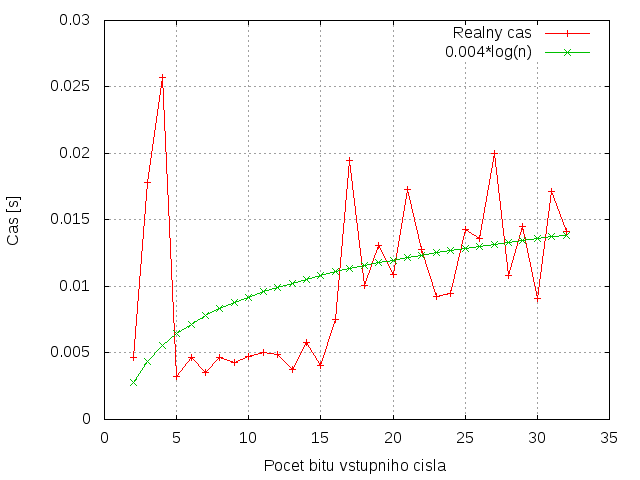
\includegraphics[scale=0.6]{perf.png}
    \caption{Doba výpočtu v~sekundách v~závislosti na počtu bitů sčítaných čísel.}
    \label{fig:res}
\end{center}
\end{figure}

\section{Sekvenční diagram}
\label{sec:seq}
Sekvenční diagram na Obrázku \ref{fig:seq} popisuje komunikační protokol procesorů
při výpočtu.
CPU $i$ je procesor provádějící řazení (slave procesor) s~identifikační
číselm $i$ (slave procesory jsou indexovány od jedné).
Číslo $n$ udává počet bitů sčítanců po případném rozšířením nulami, a tedy
i počet slave procesorů.
CPU master je procesor provádějící čtení vstupu.
Tento procesor má identifikační číslo $0$.

\begin{figure}[bt]
\begin{center}
    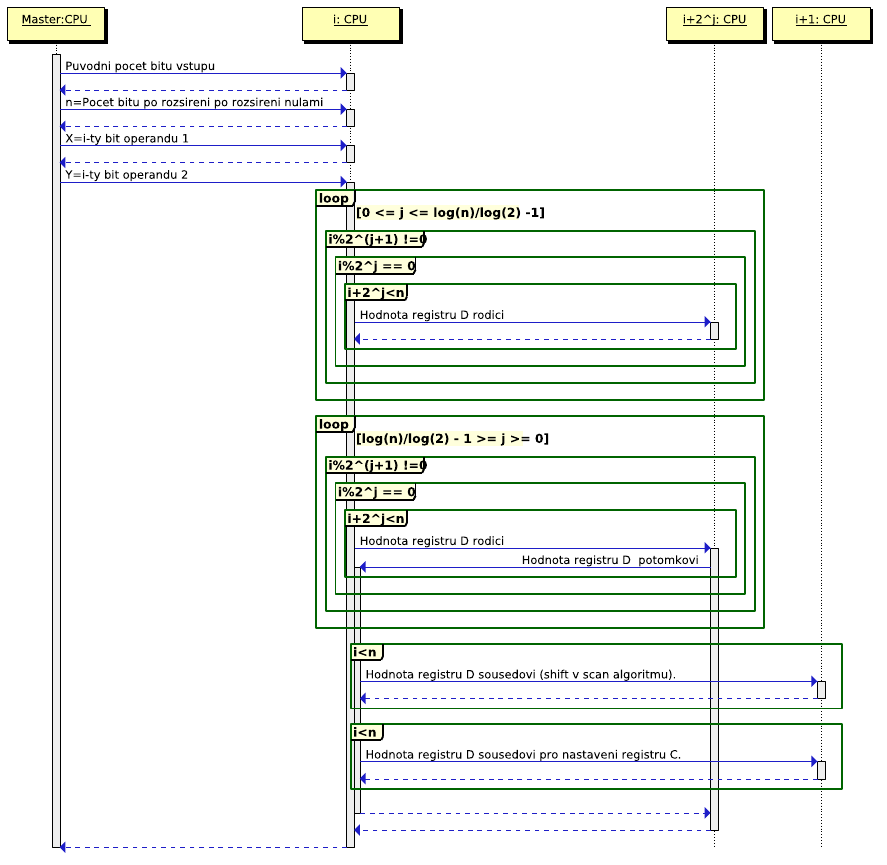
\includegraphics[scale=0.65]{seq.png}
    \caption{Sekvenční diagram zobrazující komunikační protokol procesorů.}
    \label{fig:seq}
\end{center}
\end{figure}

\section{Závěr}
V~tomtu dokumentu byl popsán algoritmus \emph{Carry Look Ahead Parallel Binary Adder}.
Následně byla provedena analýza jeho časové složitosti a ceny.
Algoritmus byl implementován a byly provedeny experimenty,
které potvrdily logaritmickou časovou složitost výpočtu odvozenou formálně,
alespoň na vzorku dat, jež byl možný testovat.
Dokument také obsahuje sekvenční diagram popisující komunikační protokol procesorů
při výpočtu algoritmu \emph{Carry Look Ahead Parallel Binary Adder}.
\end{document}
